\chapter{Obiekt regulacji}
\label{cha:ch2_obiekt_regulacji}

Obiektem poddawanym regulacji był system typu kulka na belce, który został zbudowany od podstaw na potrzeby tej pracy.

%%%%%%%%
\section{Obiekty typu kulka na belce}

Na system tego typu składają się długa, umieszczona horyzontalnie belka, łożyskowana w sposób umożliwiający zmianę kąta nachylenia, i silnik lub serwomechanizm, który umożliwia wychylanie belki.
Po belce swobodnie toczy się kulka.

Podstawowym zadaniem regulacji w systemie tego typu jest stabilizacja położenia kulki w wybranym punkcie.
Charakterystyczną cechą tego systemu jest prostota konstrukcji oraz niestabilność przy braku aktywnej regulacji.

Obiekty tego typu są często wykorzystywane w dydaktyce teorii sterowania. Składają się na to poniższe powody:

\begin{itemize}
	\item prostota budowy,
	\item możliwość zastosowania różnych czujników położenia kulki,
	\item możliwość zastosowania różnych silników i mechanizmów przeniesienia napędu,
    \item możliwość zastosowania różnych struktur i algorytmów sterowania.
\end{itemize}

Uproszczony schemat systemu kulka i belka przedstawiony został na rysunku \ref{fig:schemat_uproszczony}:

\begin{figure}[H]
	\centering
    \includesvg[width=0.6\textwidth,svgpath=./vector_graphics/]{schemat_uproszczony}
	\caption{Uproszczony schemat systemu typu kulka i belka.}
	\label{fig:schemat_uproszczony}
\end{figure}

Prostota konstrukcji i inherentna niestabilność sprawiły, że powstało wiele implementacji tego systemu (np. \cite{BABEX1}\cite{BABEX2}\cite{BABEX3}), również komercyjne, jak na przykład produkt firmy Quanser (\cref{fig:quanser_ball_beam}):

\begin{figure}[H]
	\centering
	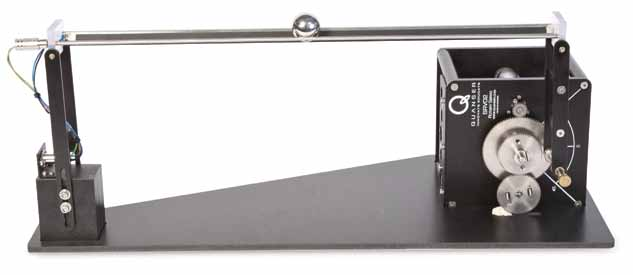
\includegraphics[width=0.5\textwidth]{quanser_ball_beam}
	\caption{Zdjęcie produktu \textit{Ball and Beam} firmy Quanser. Źródło: \url{http://www.quanser.com/Products/ball_beam}.}
	\label{fig:quanser_ball_beam}
\end{figure}

%%%%%%%%
\section{Projekt mechaniczny}

Przed przystąpieniem do budowy obiektu, zaprojektowano wstępny kształt w programie  \texttt{SketchUp Make} (\cref{fig:cad_render}). Wyszczególniono na nim:

\begin{itemize}
	\item prostokątną podstawę,
	\item słupy podtrzymujące belkę,
	\item usztywniający łącznik między słupami,
	\item oś obrotu (wał) umieszczony w połowie długości belki,
	\item przekrój belki.
\end{itemize}

\begin{figure}[H]
	\centering
	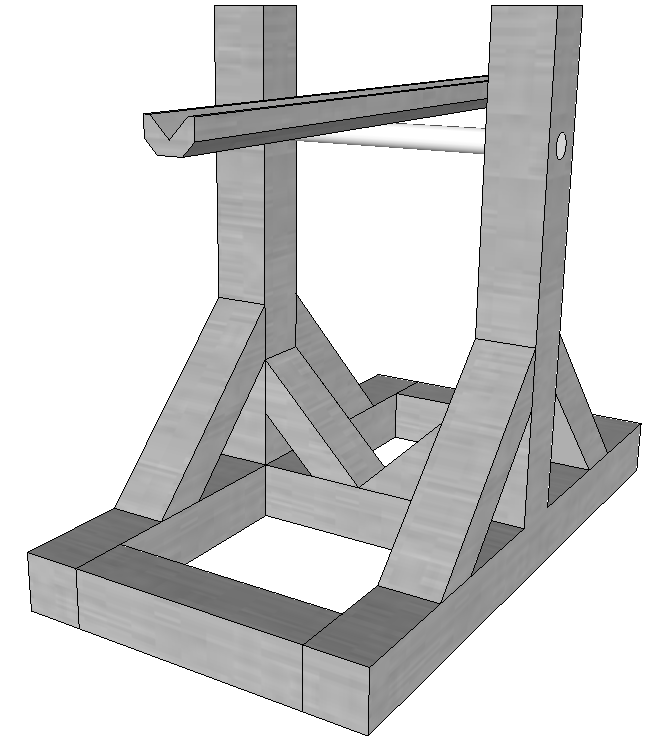
\includegraphics[width=0.3\textwidth]{cad}
	\caption{Render projektu CAD.}
	\label{fig:cad_render}
\end{figure}

Ostateczna konstrukcja różni się względem projektu \textsc{CAD} o wysokość słupów, i umiejscowienie łącznika między nimi. Dodatkowo zastosowano sztywne połączenie osi obrotu belki i samej belki wykorzystujące podpory wału.

%%%%%%%%
\section{Konstrukcja mechaniczna}
\label{sec:ch2_konstrukcja_mechaniczna}

Większość konstrukcji (\cref{fig:perspektywa}) powstała z ocynkowanych elementów stalowych, tzw. ceowników w przekroju kwadratowym o boku długości \SI{4}{cm}, pozwalających na łatwe łączenie kilku elementów przy pomocy śrub. Rozwiązanie to jest bardzo tanie w porównaniu do przemysłowych profili aluminiowych lub spawanych profili stalowych, ale jednocześnie jest dość ciężkie i poprzez niedomknięcie profilu podatne na pewne momenty gnące.

Kąty proste pomiędzy elementami ustawionymi prostopadle zostały zapewnione poprzez zastosowanie kątowych wsporników stalowych.

\begin{figure}[H]
	\centering
	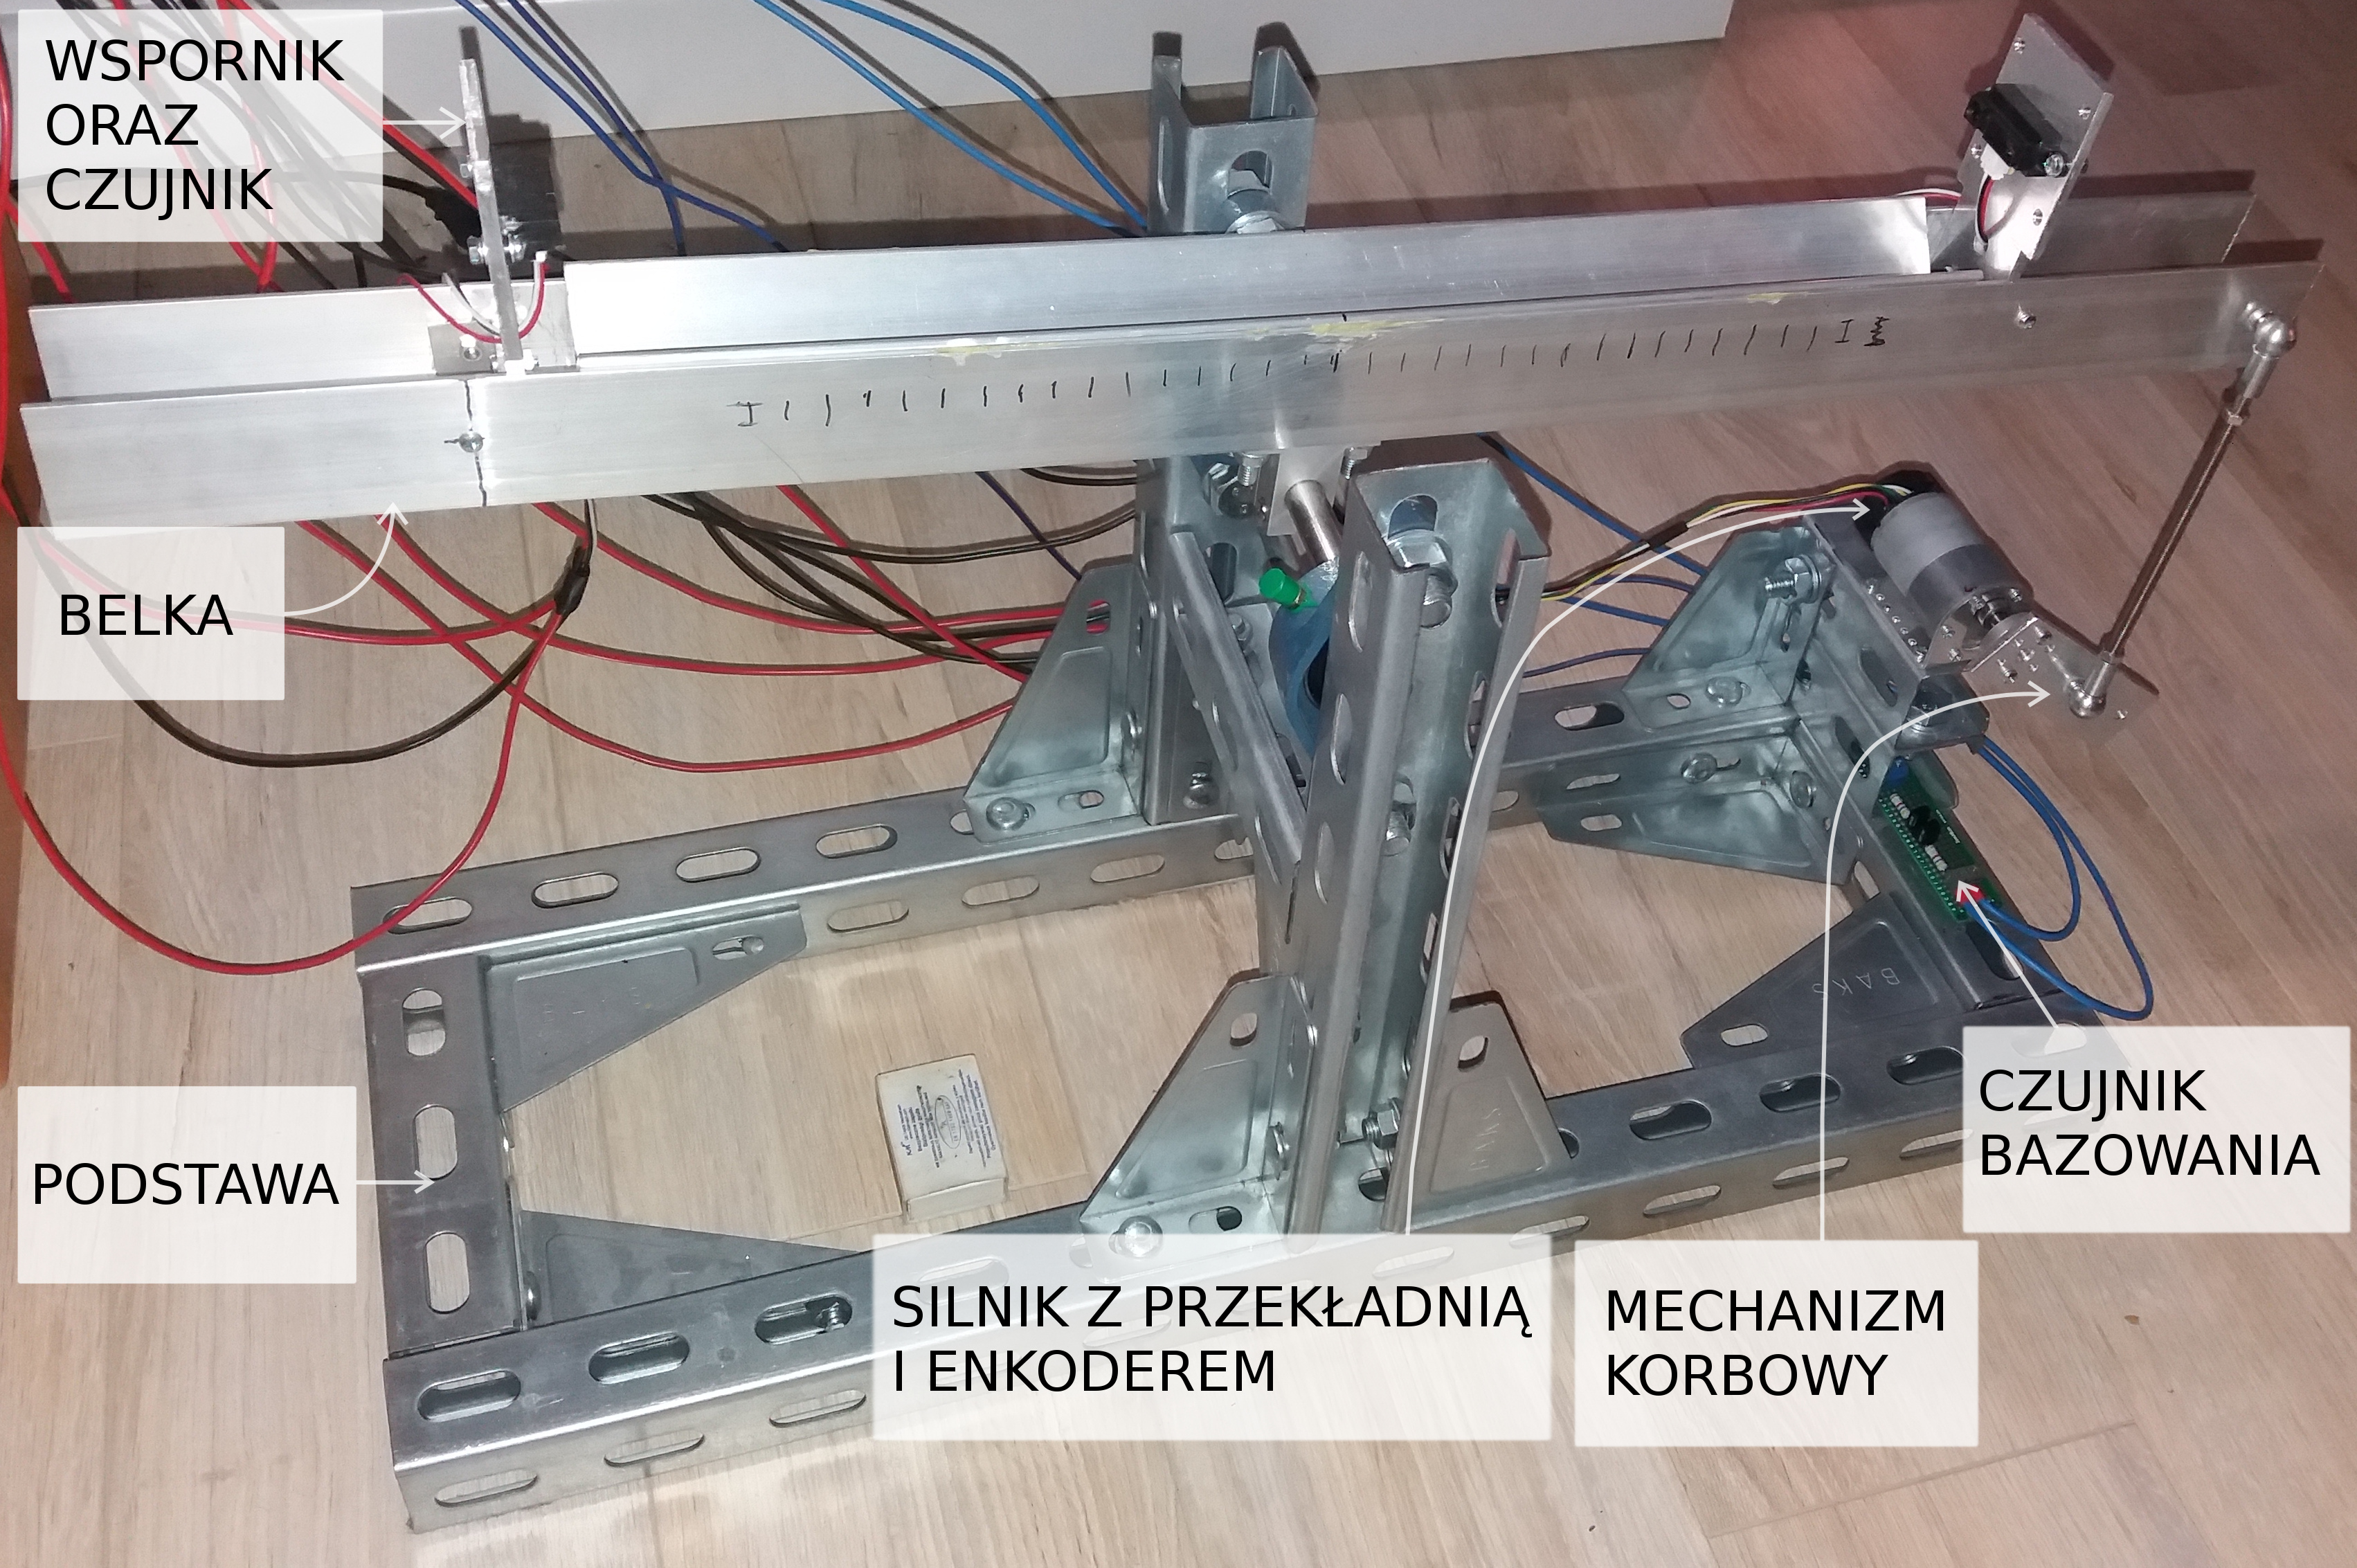
\includegraphics[width=0.9\textwidth]{perspektywa}
	\caption{Zdjęcie obiektu regulacji z zaznaczonymi poszczególnymi elementami konstrukcji; w środku obiektu opakowanie zapałek dla perspektywy.}
	\label{fig:perspektywa}
\end{figure}

Na prostokątnej podstawie o wymiarach zewnętrznych \SI{60 x 23}{cm} wykonanej z ceowników ustawiono pionowo na środkach dłuższych boków słupy nośne, również wykonane z ceowników. Słupy zostały usztywnione poprzez połączenie ich przęsłem podniesionym o \SI{11}{cm} względem podstawy.

Na słupach przyczepiono współosiowo łożyska maszynowe samonastawne typu UCFL 201 w obudowach odlewanych. Przez łożyska poprowadzono pręt nierdzewny stalowy o średnicy \SI{12}{mm}; na pręt nałożono podpory wałka w kształcie litery \texttt{T}, a do nich przykręcono belkę.

Silnik elektryczny, przymocowany do aluminiowego uchwytu, został umieszczony podłużnie na krótszym boku podstawy, na podwyższeniu wykonanym z dwóch elementów stalowych typu ceownik.

% TODO: podwyższenie zostało wzmocnione przeciwko gięciom poprzecznym i wzdłużnym poprzez zastosowanie …………

%%%%%%%%
\section{Przeniesienie napędu}
\label{sec:ch2_przeniesienie_napedu}

W obiekcie zastosowano przeniesienie napędu wykorzystujące mechanizm korbowy. Rozwiązanie to posiada kilka zalet:

\begin{itemize}
	\item gwarantuje bezpieczeństwo mechanizmu --- błąd algorytmiczny (np. przypadkowe podanie maksymalnego sterowania) nie spowoduje uszkodzenia fizycznego żadnej części obiektu,
	\item poprzez oddalenie punktu zaczepu korbowodu od osi obrotu belki zmniejsza wymagania dotyczące mocy silnika, a tym samym jego cenę,
	\item pozwala regulować zakres wychyleń belki w wyniku zmiany długości korby.
\end{itemize}

\begin{figure}[H]
	\centering
	\includesvg[width=0.6\textwidth,svgpath=./vector_graphics/]{mechanizm_korbowy}
	\caption{Schemat napędu opartego o mechanizm korbowy.}
	\label{fig:mechanizm_korbowy}
\end{figure}

Parametry fizyczne mechanizmu korbowego:

\begin{itemize}
	\item długość korby: \SI{3}{cm},
	\item długość korbowodu: \SI{16}{cm},
	\item zastosowane przeguby kulowe między korbą i korbowodem oraz korbowodem i belką,
    \item użyty silnik prądu stałego, komutatorowy, z magnesami trwałymi, sprzężony z zębatą przekładnią redukcyjną (więcej w rozdziale \ref{sec:ch3_uklad_napedowy}).
\end{itemize}

%%%%%%%%

\section{Belka}
\label{sec:ch2_belka}

Belka została stworzona poprzez trwałe sklejenie krawędzi kątownika aluminiowego o długości \SI{40}{cm} i boku \SI{3}{cm} oraz krawędzi ceownika aluminiowego o długości \SI{65}{cm} i boku \SI{4}{cm}. W przekroju przypomina to kształtem literę \texttt{M} domkniętą od spodu (\cref{fig:przekroj_belki}).

\begin{figure}[H]
	\centering
	\includesvg[width=0.2\textwidth,svgpath=./vector_graphics/]{przekroj_belki}
    % 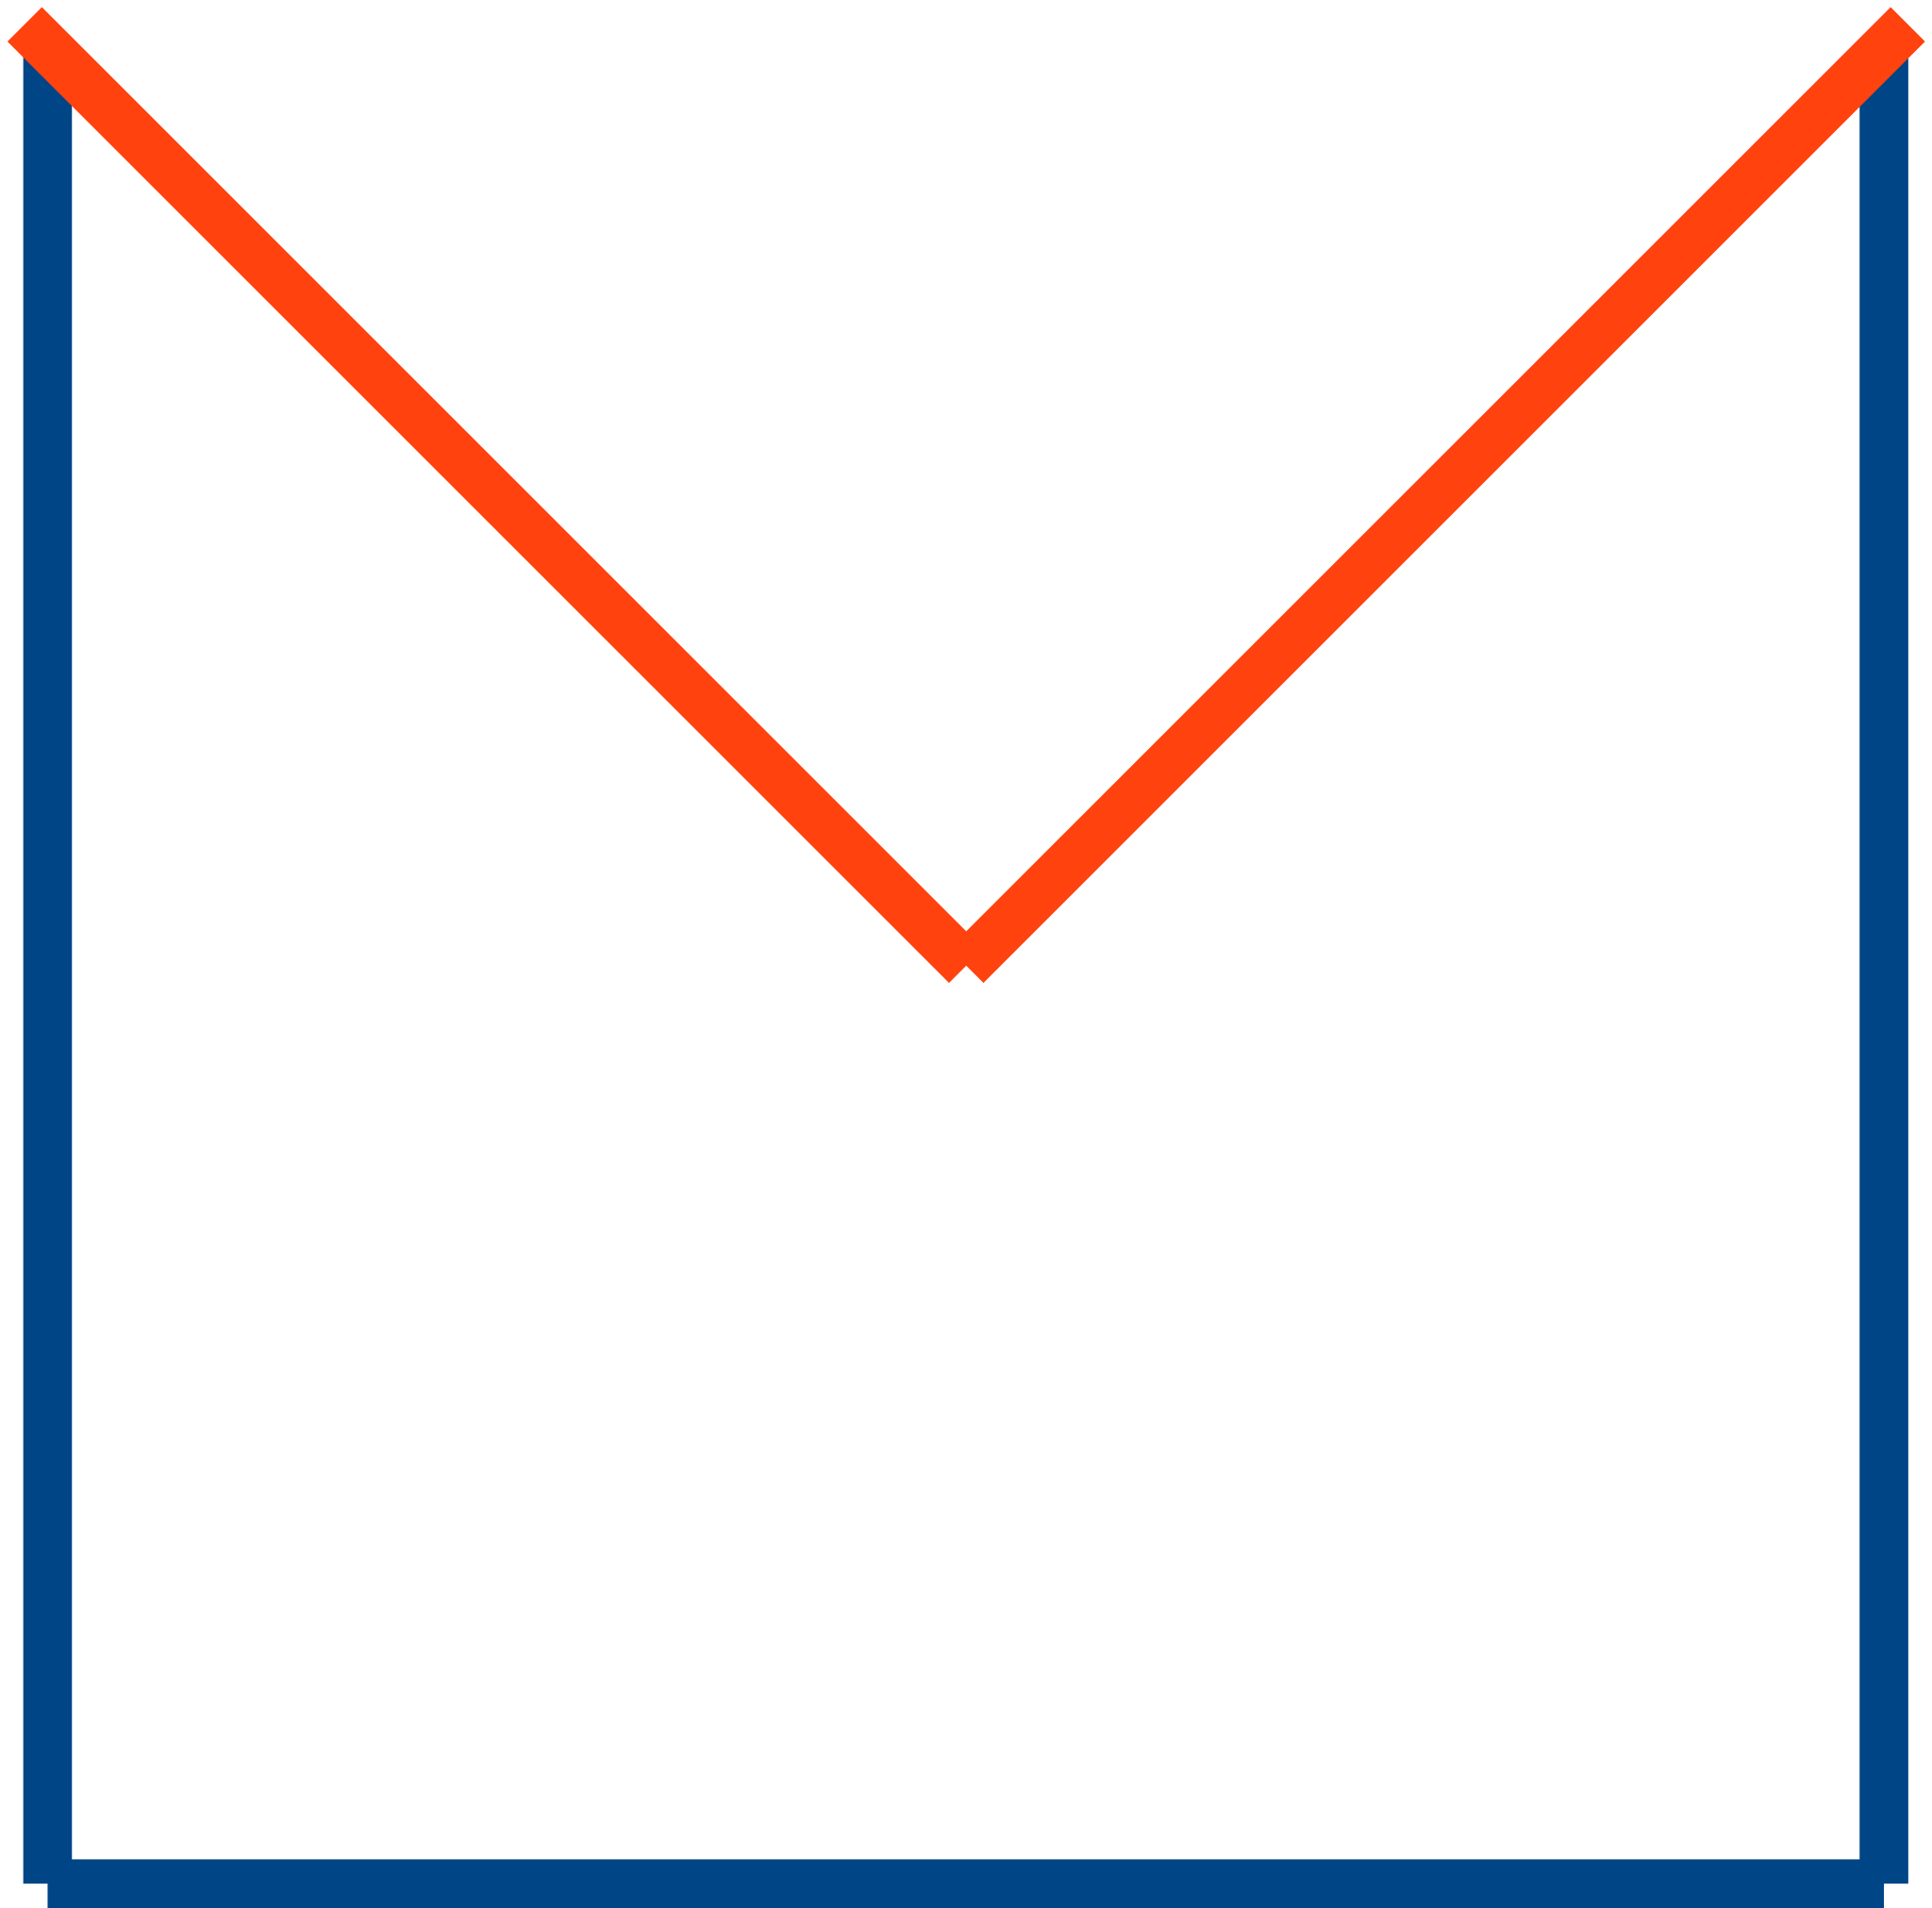
\includegraphics[width=0.2\textwidth]{beam_xsection}
	\caption{Schemat przekroju belki z zaznaczonymi ceownikiem aluminiowym A) i~kątownikiem aluminiowym B).}
	\label{fig:przekroj_belki}
\end{figure}

Użyty kątownik jest nieco krótszy od ceownika. Zamocowano go symetrycznie, a w odległościach około \SI{1}{cm} od jego końców zamontowano wsporniki (\cref{fig:uchwyt_czujnika_odleglosci}) na czujniki optyczne (zob. rozdział \ref{sec:ch3_czujniki_odleglosci}).

Wsporniki pozwalają na zmianę wysokości czujnika względem płaszczyzny belki, a także na pochylenie go w osi prostopadłej do płaszczyzny belki.

\begin{figure}[H]
    \centering
    \includesvg[width=0.4\textwidth,svgpath=./vector_graphics/]{wspornik_czujnika}
    \caption{Schemat uchwytu na czujnik odległości w rzucie od przodu i z boku. Zastosowanie mocowania na śrubie pozwala pochylać czujnik względem belki.}
    \label{fig:uchwyt_czujnika_odleglosci}
\end{figure}

%%%%%%%%
\section{Kulka}
\label{sec:ch2_kulka}

Do projektu dobrano lekką kulkę o masie \SI{20}{g} wykonaną z miękkiej pianki; średnica kulki wynosi \SI{6}{cm}.

\begin{figure}[H]
    \centering
    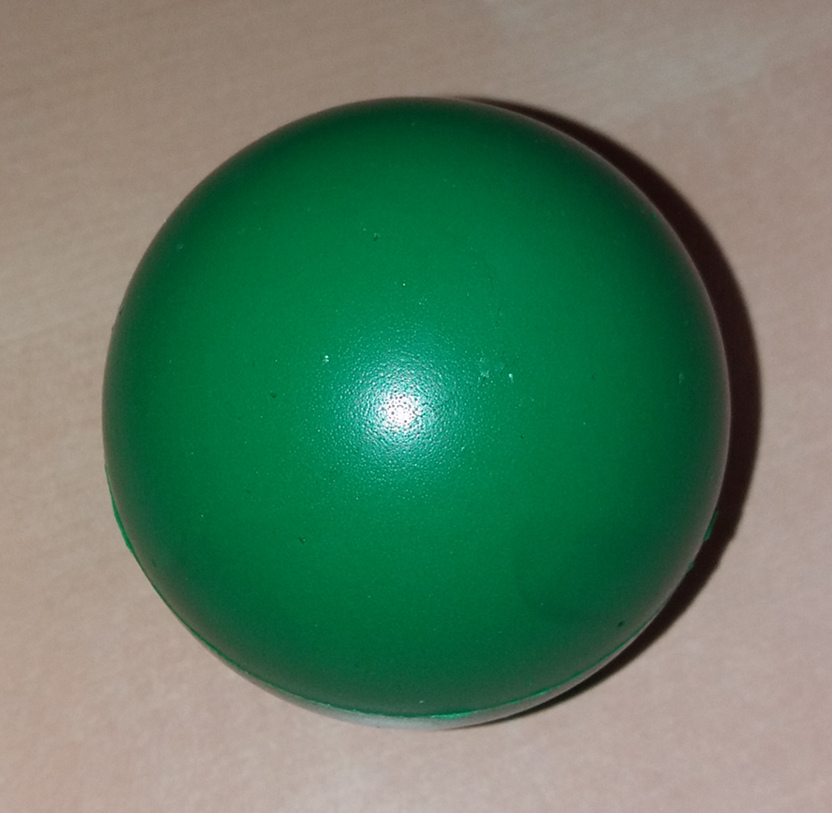
\includegraphics[width=0.4\textwidth]{ball}
    \caption{Zdjęcie kulki.}
    \label{fig:kulka}
\end{figure}

%%%%%%%%
\section{Podsumowanie}

W niniejszym rozdziale przedstawiono obiekt regulacji, cel regulacji oraz przedstawiono podobne konstrukcje, w tym jedno rozwiązanie komercyjne. Następnie opisano dokładnie budowę obiektu regulacji, poczynając od konstrukcji podstawy, poprzez umocowanie osi obrotu belki, umieszczenie silnika, przeniesienie napędu, a na budowie belki i doborze kulki kończąc.

%---------------------------------------------------------------------------